 % The main file for CAMP reports
 % Don't put any content in here. 
 % Don't even include content files by using \input or \inlcude. 
 % Put your content to TEXT.TEX or include it there using \input.
 % Uses:
 %		SETTINGS.TEX	contains the settings for this document
 %		COMMANDS.TEX	contains commands which can be used while writing
 %		INFO.TEX			contains the author, title and so on for the cover
 %		COVER.TEX			formats the front cover of the document
 %		ABSTRACT.TEX	contains the abstract to be included (if needed)
 %		TEXT.TEX			contains the actual content of the document
 %		BIB.BIB				containt the BibTeX entries for the document
 
 
%% Draft document mode
%% Final document
\documentclass[11pt,a4paper,bibtotoc,idxtotoc,headsepline,footsepline,footexclude,BCOR12mm,DIV13]{scrbook}

%\documentclass[11pt,a4paper,bibtotoc,idxtotoc,headsepline,footsepline,footexclude,BCOR20mm,DIV10]{scrbook}

% KOMA-Optionen:
%  bibtotoc: include bibliography in table of contents
%  idxtotoc: include index in table of contents
%  headsepline: use horizontalline under heading
%  BCOR: binding correcion (Bindungskorrektur) (e.g.: BCOR5mm)
%  DIV: Number of sheet sections (used for layout) (e.g.: DIV12) 



% include title and author information for the cover
% Set here the title, authors and other stuff to be used for the cover
% This file is used by MAIN.TEX

% set title, authors and stuff for the cover
\def\doctype{Diplomarbeit in Informatik}
\def\title{Semi-automated detection of sanitization, autehntication and declassification errors in UML state charts}
\def\titleGer{Halbautomatische Erkennung von Sanitisierungs-, Authenifizierungs- und Deklassifierungsfehlern in UML-Zusantsdiagrammen}
\def\author{Md Adnan Hossain Rabbi}
\def\date{November 15, 2015}

% text to appear in the footer
\def\footertext{}

% include settings
\input{components/settings}

% include commands
\input{components/commands}


%\makeindex
	%% inter line spacing
%\linespread{1.0}

\makeglossary
\usepackage[english]{babel}

\usepackage{tikz}
\newcommand*\circled[1]{\tikz[baseline=(char.base)]{
		\node[shape=circle,draw,inner sep=2pt] (char) {#1};}}
\usepackage{amsmath}
\usepackage{amsfonts}
\usepackage{graphicx}
\usepackage[skip=0pt]{caption}
\usepackage[colorinlistoftodos]{todonotes}
%\usepackage{algorithm}
\usepackage{algorithmicx}
\usepackage{algcompatible}
\usepackage{algpseudocode}

\usepackage{geometry}
\geometry{
	a4paper,
	total={210mm,297mm},
	left=20mm,
	right=20mm,
	top=20mm,
	bottom=20mm,
}
\usepackage{pifont}

\usepackage{listings}
\usepackage{color}
\usepackage[autostyle=true,style=english]{csquotes}
%\usepackage[T1]{fontenc}





\definecolor{dkgreen}{rgb}{0,0.6,0}
\definecolor{gray}{rgb}{0.5,0.5,0.5}
\definecolor{mauve}{rgb}{0.58,0,0.82}

\lstset{frame=tb,
	language=Java,
	aboveskip=3mm,
	belowskip=3mm,
	showstringspaces=false,
	columns=flexible,
	basicstyle={\small\ttfamily},
	numbers=none,
	numberstyle=\tiny\color{gray},
	keywordstyle=\color{blue},
	commentstyle=\color{dkgreen},
	stringstyle=\color{mauve},
	breaklines=true,
	breakatwhitespace=true,
	tabsize=3
}
\usepackage{booktabs}
\usepackage{multirow}
\setlength{\parskip}{\baselineskip}%
\usepackage{hyperref}% http://ctan.org/pkg/hyperref
\hypersetup{%
	colorlinks = true,
	linkcolor  = black
}

\begin{document}

	\frontmatter
	
	
	\input{components/cover}
%	\clearemptydoublepage
%	
%	\input{components/titlepage}
	
	
%	\input{components/cover_maschmeyer}
	\clearemptydoublepage
	
	\input{components/titlepage}
	
	
	\clearemptydoublepage


\thispagestyle{empty}
\selectlanguage{german}
	\vspace*{0.8\textheight}
	\noindent
	I assure the single handed composition of this master's thesis only supported by declared
	resources.
	Ich versichere, dass ich diese Masterarbeit selbst{\"a}ndig verfasst und nur 
	die angegebenen \\Quellen und Hilfsmittel verwendet habe.
	
	\vspace{15mm}
	\noindent
	M{\"u}nchen, den 15 November 2015 \hspace{5cm} \author
\selectlanguage{english}
\newpage
	
	\clearemptydoublepage
\phantomsection
\addcontentsline{toc}{chapter}{Acknowledgements}	


%\chapter*{Acknowledgements}

\vspace*{2cm}

\begin{center}
{\Large \bf Acknowledgments}
\end{center}

\vspace{1cm}




I would like to express my deepest appreciation to all those who helped me to complete this thesis. A special gratitude and thanks goes to my supervisor Prof. Dr. Claudia Eckert and my advisor, M.Sc. Paul Muntean, whose guidance, stimulating suggestions and encouragement, helped me in all the time of research and writing of this thesis. Without their cooperation in the last six months, this thesis could not be done smoothly.

Last but not the least, I wish to thank my family for their support and encouragement throughout my master studies.
	
	% Abstract for the TUM report document
% Included by MAIN.TEX


\clearemptydoublepage
\phantomsection
\addcontentsline{toc}{chapter}{Abstract}	





\vspace*{2cm}
\begin{center}
{\Large \bf Abstract}
\end{center}
\vspace{1cm}

Information flow vulnerabilities detection with static code analysis techniques is challenging because codes are usually unavailable during  the software design phase and
previous knowledge about what should be annotated and tracked
is needed. To detect information flow errors in UML state
charts and C code are not easy task as they can cause data leakages or unexpected program behavior. In this research it has been proposed that textual annotations used to
introduce information flow constraints in UML state charts and code which are afterwards automatically loaded by information flow checkers that check if imposed constraints hold or not. The experimental results of the selected sample scenarios show that this approach
is effective and can be further applied to other types of UML
models and programming languages as well, in order to detect
different types of vulnerabilities.

This thesis contributes to the development of a system for semi-automated detection of sanitization, authentication and declassification errors in UML state charts. A light-weight security annotation language is used in order to define information flow constraints regarding authentication, declassification and santization function errors  in UML state charts and source code. Annotation language editor is designed as eclipse
plug-in which is used to edit UML state charts and
source code files. Developed Source code generator as eclipse plug-in which is used to generate C code with header files from UML State chart. And finally experimented automatic loading and usage of textual annotations inside three new checkers.

	\tableofcontents
	
	\listoffigures
	
	\listoftables
  
  \clearemptydoublepage

\phantomsection
\addcontentsline{toc}{chapter}{Outline of the Thesis}

\begin{center}
	\huge{Outline of the Thesis}
\end{center}


%--------------------------------------------------------------------
%\section*{Part I: Introduction and Theory}

\noindent {\scshape Chapter 1: Introduction}  \vspace{1mm}

\noindent  This chapter presents an overview of the thesis and it's purposes. 

\noindent {\scshape Chapter 2: Background}  \vspace{1mm}

\noindent  This chapter describes the background informations and the essential theories needed for our research. Authentication, declassification and sanitization functionalities are also presented with example in this chapter. Scientific fundamentals 

%--------------------------------------------------------------------
%\section*{Part II: Implementation and Analysis}

\noindent {\scshape Chapter 3: Challenges and Annotation Language Extension}  \vspace{1mm}

\noindent  This chapter presents the challenges and annotation language extension for the system. Annotation language extension process and how it works are also presented inside this chapter.

\noindent {\scshape Chapter 4: Implementation}  \vspace{1mm}

\noindent  This chapter presents the implementation of the system. Implementation mechanism, technology and tools which have been used to develop the system are also presented inside this chapter.

\noindent {\scshape Chapter 5: Experiments}  \vspace{1mm}

\noindent  This chapter presents the different application areas of the system. Inside this chapter the system is checked for three real-life scenarios and presented the outcome of the system. 

\noindent {\scshape Chapter 6: Related Work}  \vspace{1mm}

\noindent  This chapter presents the some of the related work of this research. Some of the related tools that have been already developed are also presented inside this chapter.


%--------------------------------------------------------------------
%\section*{Part III: Conclusion and Future Works}

\noindent {\scshape Chapter 7: Limitations, Conclusion and Future Work}  \vspace{1mm}

\noindent  This chapter presents the limitations of this research, conclusion of the whole research along with future work intentions.

	\mainmatter
	
	
		% ---------------------------------------------------------------------------
		%
		%Introduction and Background Theory
		%
		% ---------------------------------------------------------------------------
		\part[The 1st Part]{Introduction and Theory}
		\label{part:introAndBackgroundTheory}
		\chapter{Introduction}
\label{chapter:Introduction}

The detection of information flow vulnerabilities uses dynamic analysis techniques , static analysis techniques and hybrid techniques which combine static and dynamic approaches. The static techniques need to know when to use  sanitization , declassification and authentication functions.
A solution for tagging sanitization, declassification and authentication in source code is based on libraries which contain all needed annotations attached to function declarations. This approach plays an important role mainly for static analysis bug detection techniques where the information available during program run-time is not available nor the interaction with the environment can be fully simulated.
Extended Static Checking (ESC) is a promising research area which tries to cope with the shortage of not having the program run-time information. During extended static analysis additional information is provided to the static analysis process. This information can be used to define trust boundaries and tag variables. Textual annotations are usually manually added by the user in source code. At the same time annotations can be automatically generated and inserted into source code . ESC can be used to eliminate bugs in a late stage of the software project when code development is finished. Tagging and checking for information exposure bugs during the design phase would eliminate the potential of implementing software bugs which can only be removed very costly after wards. Thus security concerns should be enforced into source code right after the conceptual phase of the project.
The paper presents five challenges concerning ESC. The last challenge reports of the annotation as being a very time consuming burden and is therefore disliked by some programming
teams. The authors argue about the fact that annotations can cover design decisions and enhance the quality of source code. We argue that annotations are necessary in order to do ESC and the user needs a kind of assistance tool that helps selecting the suited annotation based on the current context. Thus the annotation burden needed for learning and applying the language should be reduced. At the same time adding annotations to reusable code libraries reduces even more the annotation burden since libraries can be reused, shared and changed by software development
teams.
 
 \cite{haykin2004comprehensive}
\section{Latex Introduction}
There is no need for a latex introduction since there is plenty of literature out there.
 



		\chapter{Background Information}

\section{Sanitization}
Sanitization is the process of removing sensitive information from a document or other message or sometimes encrypting messages, so that the document may be distributed to a broader audience. Sometimes sanitization can be called as an operation that ensures that user input can be safely used in an SQL query. Web applications use malicious input as part of a sensitive operation without having properly checked or sanitized the input values from the user. Previous research on vulneribility analysis has mostly focused on identifying cases which web applications directly uses external input for critical operations. It is suggested that always use proper sanitization method to validate external input values from the user for any application.For example, user inputs must always flow through a sanitizing function before flowing into a SQL query or HTML, to avoid SQL injection or cross-site scripting vulnerabilities.\\

Reflection of security breaches are very significant for high assurance system. For examples of this type of systems are aircraft navigation, where a fault could lead to a crash, various control systems which has critical infrastructure , where an error 
could cause toxic waste to leak, and weapons targeting, where an inaccuracy could result in severe collateral damage. In such
operational environments, the impact is virtually irreversible and must therefore be prevented even if it is likely to occur
with low probability.It's always good that transforming information to a form which is suitable for release or sanitize the information by redacting some portions of it.\\

Some basic purpose of sanitization are given below:
\begin{itemize}
	\item Remove malicious elements from the input.
	\item To identify the set of parameters and global variables which must be sanitized before calling functions.
	\item It is acceptable to first pass the untrusted user input through a trusted sanitization function.	
	\item Any user input data must flow through a sanitization function before it flows into a SQL query.
	\item Confidential data needs to be cleansed to avoid information leaks.
	\item Most paths that go from a source to a sink pass through a sanitizer.
	\item Developers typically define a small number of sanitization functions in libraries.
\end{itemize}

\section{Declassification}
Information security has a challenge to address: enabling information flow controls with expressive information release (or declassification) policies. In a scenario of systems that operate on data with different sensitivity levels, the goal is to provide security assurance via restricting the information flow within the system. Practical security-typed languages support some form of declassification through which high-security information is allowed to flow to a low-security system or observer.\\

United States Federal Trade Commission reveals the damage that is continually caused by electronic information leakage. In protecting sensitive information, including everything from credit card information to military secrets to personal, medical information, there is a highly
need for software applications with strong, confidentiality guarantees.
Security-typed languages promise to be a valuable tool in making provably secure software applications. In such languages, each
data item is labeled with its security policy. In practical security-typed languages support some form of declassification, in which high-security information is permitted to flow to a low-security receiver/observer \\

To declassify information means lowering the security classification of selected information. Sabelfeld and Sands \cite{ref_3_sabelfeld2009declassification} identify four different dimensions of declassification, what is declassified, who is able to declassify, where the declassification occurs and when the declassification takes place.\\

Myers and Liskov introduced the decentralized label model \cite{ref_4_myers2000protecting}, describing how labels could be applied
to a programming language and then used to check information
flow policy compliance in distributed systems. The framework
includes a declassify function for downgrading data if the
owners policies allow. The model allows principals to define their own downgrading policies.\\

\subsection{Dimensions of declassification}
Classification of the basic declassification goals according to four axes: what information is released, who releases information, where in the system information is released and when information can be released.

\begin{itemize}
   \item What : Selective or Partial information flow policies \cite{ref_5_cohen1977information,ref_6_cohen1978information,ref_7_joshi2000semantic,ref_8_giacobazzi2005adjoining} regulate what
   information may be released. Partial release guarantees that only a part of a secret is
   released to a public domain. Partial release can be specified in terms of precisely which
   parts of the secret are released. This is useful,
   for example, when partial information about a credit card number or a social security number is used for logging.
   
   \item Who : In a computing system it is essential to specify who controls information release .
   Ignoring the issue of control opens up attacks where the attacker hijacks release
   mechanisms to launder secret information. Myers and Liskov decentralised label
   model \cite{ref_9_myers1997decentralized} security labels with explicit ownership information. According to this approach, information release of some data is safe if it is performed by the
   owner who is explicitly recorded in the data security label. This model has been used for enhancing Java with information flow controls \cite{ref_10_myers1999jflow} and has been implemented in
   the Jif compiler \cite{ref_11_myers2001jif}.
   
   \item Where : In a system information  Where is an important aspect of information release.One can ensure that no other  part can release further information.
   by delegating particular parts of the system to release information.Declassification
   via encryption is not harmful as long as the program is, in some sense, noninterfering
   before and after encryption.  A combination of \enquote{where} and \enquote{who} policies in the presence of encryption has
   been recently investigated by Hicks et al.\cite{ref_12_hicks2005declassification}
   
   \item When : The fourth dimension of declassification is  \enquote{when} information should be released.The work of Giambiagi and Dam [29] focuses on the correct implementation of security protocols. Here the goal is not to prove a noninterference property of the protocol, but to use the components of the protocol description as a specification of what and when information may be released.Chong and Myers security policies \cite{ref_13_chong2004security} address when information is released.By annotating variables this is achieved .
   
\end{itemize}

\section{Authentication}
Authentication is the mechanism which confirms the identity of users trying to access a system. For a user to be granted access to a resource, they must first prove that they are who they claim to be. Generally this is handled by passing a key with each request (often called an access token, User verification using user id and password). The system or server verifies that the access token or user id and password is genuine, that the user does indeed have the required privileges to access the requested resource and only then the request granted.\\
Also authentication can be defined as it is the process by which the system validates a user's logon information. A user's name and password are compared to an authorized list and if the system detects a match then access is granted to the extent specified in the permission list for that user.\\

One familiar use of authentication and authorization is access control. A computer system that is supposed to be used only by those authorized must attempt to detect and exclude the unauthorized. Common examples of access control involving authentication include:
\begin{itemize}	
	\item A computer program using a blind credential to authenticate to another program.
	\item Logging in to a computer.	
	\item Using an Internet banking system.
	\item Withdrawing cash from an ATM and more
\end{itemize}

\section{ Detecting Information Flow Errors During Design:}
If a step of function call like authentication, sanitization or declassification is missing inside the program then this can lead to software vulnerabilities. In the figure 2.1 left side picture depicted that it has three functions. Among then func2() is named either sanitization/declassification/authentication function. Which means in this scenario there will be no error regarding sanitization/declassification/authentication function. On the other hand the right side picture represents there is a missing function of sanitization/declassification/authentication function. That's why it is the buggy path of UML state charts during design stage of software life cycle. 
\begin{figure}[htbp]
	\centering
	\includegraphics{styles/FunctionCallMissing.png}
	\caption{Information flow errors during design}
\end{figure}


\section{ Detecting Information Flow Errors During Coding:}

Figure 2.2 depicts two explicit information flows according to A lattice model of secure information flow of Denning \cite{ref_14_denning1976lattice} contained in two systems (system 1) and (system 2)
where each of the flows starts with statement variable a and ends with leaving the system. The the variable declaration up to outside the system represent C language statements. System 1 is depicted in left side containing the flow from the source to the sink and leaving the system indicated with circles at the top and bottom of each of the
two information flows. A source is any function or programming language statement which provides private information through a system boundary. A sink can be a function call or programming language statement which exposes private information to the outside of the system through a system boundary. A system boundary can be a statement, function call, class, package or module. In figure 2.2 the source and sink represent C language statements where information enters and respectively leaves system 1 or system 2. The variable a was tagged with label \enquote{H} (confidential) as it inserts confidential information into system 1. The arrows represent the passing of the confidential label \enquote{H} between the program statements. When a variable labeled with \enquote{H} is about to leave system 1 or system 2 without passing through either authentication/declassifiaction/sanitization function then a bug report should be created.In figure 2 right side system has a bug because it passes a secured/confidential information without passing through authentication/declassifiaction/sanitization function. These functions either authenticated,declassified or sanitized  secured/confidential information and makes the variable label as \enquote{L} to leave the system. But in the left part of the picture there is no bug as in this system, secured/confidential information and the variable which is labeled with \enquote{H} passes through either authentication/declassifiaction/sanitization function.

\begin{figure}[htbp]
	\centering
	\includegraphics{styles/bug_detection_during_coding.png}
	\caption{Information flow errors during coding}
\end{figure}

		
		
		
		%
		%% ---------------------------------------------------------------------------
		%%
		%% Fully Automated Calibration for Ultrasound
		%%
		%%% ---------------------------------------------------------------------------
		\part[The 2nd Part]{Implementation and Analysis}
		\label{part:secondP}
		\chapter{ Challenges and Annotation Language Extension}
Main goal was to overcome the challenge of not being able
to detect implicit and explicit information flow bugs in UML state charts and C code. An annotation language
which can be used to annotate UML state charts and code by inserting information flow
restrictions during two software development phases (design
and coding). The insight was that the same annotation language can be used to add information flow constraints to UML state charts and code in order to detect information flow errors.
 
In this chapter the challenges and how the annotation language has extended are described.

\section{Challenges and Idea}

To develop the system eclipse xtext, eclipse xtend and static analysis engine named smtcodan(which is developed in Java to detect C and C++ vulneribilities) are used. For building the source code annotation editor eclipse xtext is used. Modeling the source as UML Statechart opensource platform YAKINDU SCT editor is used. Inside YAKINDU sct editor to genrate the .c(c file) and .h(header file) eclipse xtend is used mainly for genrating code files from statechart. Let's see in briefly what is xtext, xtend and how it works.

\begin{itemize}	
	\item Xtext : Xtext is a framework for development of programming languages and domain specific languages.According to the \cite{ref_17_xtext:grammar}, it covers all aspects of a complete language infrastructure, from parsers, over linker, compiler or interpreter to fully-blown top-notch Eclipse IDE integration. It comes with great defaults for all these aspects which at the same time can be easily tailored to your individual needs.
	Here is an example of Xtext file:
		\begin{lstlisting}
		grammar org.xtext.example.mydsl.MyDsl with 
		org.eclipse.xtext.common.Terminals
		
		generate myDsl "http://www.xtext.org/example/mydsl/MyDsl"
		
		Model:
		messages+=Message*;
		
		Message:
		'Hello' name=ID '!';
		
		\end{lstlisting}
		 
	This language allows to write down a list of messages. The following would be proper input messages which are allowed to write:
		\begin{lstlisting}
			Hello User!
			Hello World!		
		\end{lstlisting}
		
	\textbf{How Xtext Works:}
	Xtext provides user with a set of domain-specific languages and modern APIs to describe the different aspects of user's programming language. Based on that information it gives user a full implementation of that language running on the JVM. The compiler components of user's language are independent of Eclipse or OSGi and can be used in any Java environment. They include such things as the parser, the type-safe abstract syntax tree (AST), the serializer and code formatter, the scoping framework and the linking, compiler checks and static analysis aka validation and last but not least a code generator or interpreter. These runtime components integrate with and are based on the Eclipse Modeling Framework (EMF), which effectively allows user to use Xtext together with other EMF frameworks like for instance the Graphical Modeling Project GMF.
	
	In addition to this nice runtime architecture, user will get a full blown Eclipse-IDE specifically tailored for user's language. It already provides great default functionality for all aspects and again comes with DSLs and APIs that allow to configure or change the most common things very easily. And if that's not flexible enough there is Guice to replace the default behavior with user's own implementations.
	
	\textbf{Domain-Specific Language:}
	A Domain-Specific Language (DSL) is a small programming language, which focuses on a particular domain. Such a domain can be more or less anything. The idea is that its concepts and notation is as close as possible to what you have in mind when you think about a solution in that domain. 
		
	The opposite of a DSL is a so called GPL, a General Purpose Language such as Java or any other common programming language. With a GPL you can solve every computer problem, but it might not always be the best way to solve it.
	
	Imagine you want to remove the core from an apple. You could of course use a Swiss army knife to cut it out, and this is reasonable if you have to do it just once or twice. But if you need to do that on a regular basis it might be more efficient to use an apple corer.
	
	There are a couple of well-known examples of DSLs. For instance SQL is actually a DSL which focuses on querying relational databases. Other DSLs are regular expressions or even languages provided by tools like MathLab. Also most XML languages are actually domain-specific languages. The whole purpose of XML is to allow for easy creation of new languages. Unfortunately, XML uses a fixed concrete syntax, which is very verbose and yet not adapted to be read by humans. Into the bargain, a generic syntax for everything is a compromise.
	
	Xtext is a sophisticated framework that helps to implement your very own DSL with appropriate IDE support. There is no such limitation as with XML, you are free to define your concrete syntax as you like. It may be as concise and suggestive as possible being a best match for your particular domain. The hard task of reading your model, working with it and writing it back to your syntax is greatly simplified by Xtext.
	
	\textbf{Users of Xtext:}
	Xtext is used in many different industries. It is used in the field of mobile devices, automotive development, embedded systems or Java enterprise software projects and game development. People use Xtext based languages to drive code generators that target Java, C, C++, C sharp, Objective C, Python, or Ruby code. Although the language infrastructure itself runs on the JVM, you can compile Xtext languages to any existing platform. Xtext based languages are developed for well known Open-Source projects such as Maven, Eclipse B3, the Eclipse Webtools platform or Google's Protocol Buffers and the framework is also widely used in research projects.
	
	\item Xtend : According to the \cite{ref_20_xtend}, Xtend is a statically-typed programming language which translates to comprehensible Java source code. Syntactically and semantically Xtend has its roots in the Java programming language but improves on many aspects such as- Extension methods, Lambda Expressions, Active Annotations, Operator overloading, Powerful switch expressions, Multiple dispatch, Template expressions etc. Xtend has zero interoperability issues with Java: Everything you write interacts with Java exactly as expected. At the same time Xtend is much more concise, readable and expressive. Its small library is just a thin layer that provides useful utilities and extensions on top of the Java Development Kit (JDK). 
	
	\textbf{Java Interoperability:}
	Xtend, like Java, is a statically typed language. In fact it completely supports Java's type system, including the primitive types like int or boolean, arrays and all the Java classes, interfaces, enums and annotations that reside on the class path.
	
	Java generics are fully supported as well: You can define type parameters on methods and classes and pass type arguments to generic types just as you are used to from Java. The type system and its conformance and casting rules are implemented as defined in the Java Language Specification.
	
	Resembling and supporting every aspect of Java's type system ensures that there is no impedance mismatch between Java and Xtend. This means that Xtend and Java are 100\% interoperable. There are no exceptional cases and you do not have to think in two worlds. You can invoke Xtend code from Java and vice versa without any surprises or hassles. As a bonus, if you know Java's type system and are familiar with Java's generic types, you already know the most complicated part of Xtend.
	
	The default behavior of the Xtend to Java compiler is to generate Java code with the same language version compatibility as specified for the Java compiler in the respective project. This can be changed in the global preferences or in the project properties on the Xtend  Compiler page (since 2.8). Depending on which Java language version is chosen, Xtend might generate different but equivalent code. For example, lambda expressions are translated to Java lambdas if the compiler is set to Java 8, while for lower Java versions anonymous classes are generated.
	
	\textbf{Type Inference:}
	One of the problems with Java is that you are forced to write type signatures over and over again. That is why so many people do not like static typing. But this is in fact not a problem of static typing but simply a problem with Java. Although Xtend is statically typed just like Java, you rarely have to write types down because they can be computed from the context.
	
	Consider the following Java variable declaration:
	\begin{lstlisting}
		final LinkedList<String> list = new LinkedList<String>();
	\end{lstlisting}
	The type name written for the constructor call must be repeated to declare the variable type. In Xtend the variable type can be inferred from the initialization expression:
	\begin{lstlisting}
		val list = new LinkedList<String>
	\end{lstlisting}
		
	Here is an example of Xtend file:
	\begin{lstlisting}
	package example	
	import java.util.List		
	class A {
	def greetToAll(List<String> names) {
		for(name: names) {
			println(name.helloMessage)
		}
	}
		
	def helloMessage(String name) {
		'Hello ' + name + '!'
		}
	}
	
	\end{lstlisting} 
	   
Xtend provides type inference, the type of name and the return types of the methods can be inferred from the context. Classes and methods are public by default, fields private. Semicolons are optional.
	
The example also shows the method helloMessage called as an extension method, like a feature of its first argument. Extension methods can also be provided by other classes or instances.
\end{itemize}


Previous annotation language grammer has been extended more
to detect implicit and explicit information flow bugs in UML
state charts and C code. The purpose of the same annotation language
can be used to add information flow constraints to UML state
charts and code in order to detect information flow errors.\\

The challenge was addressed by extending the annotation language containing textual annotations which can be used to annotate source code and UML state charts which are backward compatible.The single-line annotations have the same as previous consisting start tag "//@" and the multi-line annotations have the start tag "/*@" and the end tag "@*/" .\\

Some challenges throughout the approach are- converting textual
comments into annotations objects, introducing syntactically
correct annotations into files, how to use the same annotation
language in order to annotate UML state charts and source
code, dealing with scattered annotations and attaching annotations to the right function declaration or variable.\\

The eclipse xtext based grammar is used to parse the whole C/C++ language. The C/C++ source code file extensions (.h, .hh, .hhh, .hxx, .c, .cpp) and UML state chart annotation box (graphical boxes
which can be attached to different parts of a UML state chart diagram) can be annotated with policy language restrictions. The obtained CORE model (a one to one mapping from xtext grammar to the ECORE grammar representation) that can be reused for integrating the policy language into an UML state chart editor. Treating the annotation tags as EObjects created new possibilities for annotating
UML models.The policy language grammar has about 420 lines of code with code comments included. Source code generation is also supported by using
eclipse xtend, ANTLR and .mwe2 files. To parse other programming languages as well this annotation language parser can be used.The result is an extensible policy language and a highly reusable source code implementation as well as source code generator that can easily be used for annotating models and source files.

\section{Annotation Language Tags}
Table \ref{table:Security_language_annotation_tags} contains in this section: the annotation language
target types, the annotation tags which can be used in
combination with the tag @function, the tag
@parameter can be used to annotate the function parameter as authinticated/declassified/santized H/L and the tag @variable used to annotate the variable of C/C++ code with confiential H/L which are used to tag public and private variables. The tag @variable which can be used only inside single line annotations whereas @parameter is used only in multi line annotations. The tags were
defined and implemented iteratively based on the work flow
presented in figure \ref{figure:Language_Design_Process} and by using the eclipse xtext \cite{ref_17_xtext:grammar} language
definition grammar.\\

For detecting of authentication, declassification and sanitization errors new function tags included like authentication, declassification and sanitization function type. Also for parameter new tag type of parameter included such as authenticated, declassified and sanitized. Still H/L tags for parameter exists in the annotation tags for parameter to define that which type of parameter is this either \enquote{High} or \enquote{Low}. High means that this parameter is highly confidential or secured and low means that this parameter is not highly secured. The tag preStep used to annotate the previous function call name and tag postStep is used for next function call name. In Table \ref{table:Security_language_annotation_tags} the new tags for annotation language grammar has given with previous annotation tags. 

\begin{table}
	\centering
\begin{tabular}{l*{3}{c}r}
	\hline
	Annotation Type   & Annotation Tag & Description  \\
	\hline

	@function         & sink  		   & uses information \\
	                  & source         & source provides information	\\
	                  & authentication & authentication authenticates information	\\
	                  & declassification& declassification declassifies information	\\
	                  & sanitization   & sanitization sanitizes information	\\
	                  & trust\_boundary& trust\_boundary is a trust-boundary\\ \hline

	@parameter        & authenticated H/L & authenticated High/Low tags    \\
					  & declassified H/L  & declassified High/Low tags    \\
				      & sanitized H/L     & sanitized High/Low tags    \\ \hline
	@variable         & confidential H/L & confidential High/Low tags\\
					  & source H/L & source High/Low tags   \\
	\hline
	
	@preStep         & preStep  & previous function call name\\ 	\hline
	@postStep        & postStep  & next function call name\\ 	\hline

	
\end{tabular}
\caption{Security language annotation tags}
\label{table:Security_language_annotation_tags}
\end{table}

\section{Annotation Language Implementation Process}

To implement the annotation language Eclipse Xtext \cite{ref_17_xtext:grammar} was used. Xtext is a sophisticated framework that helps to implement own DSL(Domain Specific Language) with appropriate IDE support. There is no such limitation as with XML, user's are free to define user's concrete syntax as user like. It may be as concise and suggestive as possible being a best match for user's particular domain. The hard task of reading user model, working with it and writing it back to user's syntax is greatly simplified by Xtext. Xtext relies heavily on Eclipse Modeling Framework (EMF) internally, but it can also be used as the serialization back-end of other EMF-based tools.  

Xtext provides a lot of generic implementations for language's infrastructure but also uses code generation to generate some of the components. Those generated components are for instance the parser, the serializer, the inferred Ecore model (if any) and a couple of convenient base classes for content assist etc.The generator also contributes to shared project resources such as the plugin.xml, MANIFEST.MF and the Guice modules. Xtext's generator uses a special DSL called MWE2 - the modeling workflow engine to configure the generator. MWE2 allows to compose object graphs declaratively in a very compact manner. The nice thing about it is that it just instantiates Java classes and the configuration is done through public setter and adder methods as one is used to from Java Beans encapsulation principles.

Xtext itself and every language infrastructure developed with Xtext is configured and wired-up using dependency injection. Xtext may be used in different environments which introduce different constraints. Especially important is the difference between OSGi managed containers and plain vanilla Java programs. To honor these differences Xtext uses the concept of ISetup (src)-implementations in normal mode and uses Eclipse's extension mechanism when it should be configured in an OSGi environment.

The Modeling Workflow Engine 2 (MWE2) is a rewritten backwards compatible implementation of the Modeling Workflow Engine (MWE). It is a declarative, externally configurable generator engine. Users can describe arbitrary object compositions by means of a simple, concise syntax that allows to declare object instances, attribute values and references. One use case - that's where the name had its origins - is the definition of workflows. Such a workflow consists usually of a number of components that interact with each other. There are components to read EMF resources, to perform operations (transformations) on them and to write them back or to generate any number of other artifacts out of the information. Workflows are typically executed in a single JVM. However there are no constraints the prevent implementors to provide components that spawn multiple threads or new processes.

Xtext ships with a default set of predefined, reasonable and often required terminal rules. The grammar for these common terminal rules is defined as follows:
	\begin{lstlisting}
		grammar org.eclipse.xtext.common.Terminals 
		hidden(WS, ML_COMMENT, SL_COMMENT)
		import "http://www.eclipse.org/emf/2002/Ecore" as ecore
		terminal ID : 
		'^'?('a'..'z'|'A'..'Z'|'_')('a'..'z'|'A'..'Z'|'_'|'0'..'9')*;
		terminal INT returns ecore::EInt: 
		('0'..'9')+;
		terminal STRING  : 
		'"' ( '\\'('b'|'t'|'n'|'f'|'r'|'u'|'"'|"'"|'\\') | !('\\'|'"') )* '"' |
		"'" ( '\\'('b'|'t'|'n'|'f'|'r'|'u'|'"'|"'"|'\\') | !('\\'|"'") )* "'"; 
		terminal ML_COMMENT  : 
		'/*' -> '*/';
		terminal SL_COMMENT : 
		'//' !('\n'|'\r')* ('\r'? '\n')?;
		terminal WS  : 
		(' '|'\t'|'\r'|'\n')+;
		terminal ANY_OTHER: 
		.;
	\end{lstlisting}

In order to implement the annotation language grammer in this research it was required to extend the terminal rule ML\_COMMENT and SL\_COMMENT. After extending these two rules it looks like this:

\begin{lstlisting}
	/**
	* @SL_COMMENT :all strings which follow // | || | } will be a single line comment
	*/ 
	terminal SL_COMMENT 	: '//'!('@')  !('\n'|'\r')* ('\n'|'\r')*
	// '}' can be used optional to disable the method bodyes together with multiline line {} comment 
	//     | '}'         !('\n'|'\r')* ('\n'|'\r')*               
	;
	
	/**
	* @ML_COMMENT :@/* multiline comment excluding @ from inside
	*            :{} multi line comment 
	*/ 
	terminal ML_COMMENT	: '/*' !('@') -> !('@')'*/'   !('\n'|'\r')* ('\n'|'\r')*   
	// '{' -> '}' can be used optional to disable the method bodyes together with single line { comment 
		//      | '{' -> '}'                   ('\n'|'\r')?
		;   
\end{lstlisting}

The process depicted in figure \ref{figure:Language_Design_Process} was used in order to
implement annotation language. Figure 3.1 depicts the
annotation language implementation process. The process is
comprised of the following steps: At first, the .xtext file
containing the language grammar was extended following the requirements. Next the grammar file is compiled and software artifacts are generated. After editing the .mwe2 file then compile it. The result of compiling is: a parser, a lexer and class bindings between these two (lexer and parser) and the grammar ECore model. The generated parser, lexer and the bindings were reused inside static analysis engine and in the UI source file editor. After opening and editing a source file with the editor,the file can be parsed and the annotations can be automatically loaded and used inside checkers.
\begin{figure}[htbp]
	\centering
	\includegraphics{styles/Language_Design_Process.png}
	\caption{Annotation language design process}
	\label{figure:Language_Design_Process}
\end{figure}
		\chapter{Implementation}

\section{Complete Workflow of the System:}




\section{The Grammar of Annotation Language:}

As per requirements previous annotation language grammar which is written in xtext language has been extended. Extra annotation have included like "@return", "True", "False", "sanitization", "declassification", "authentication". Some the code snippet of extended xtext grammar is given below.
\begin{lstlisting}
	/**
	* @FunctionAnnotation :used for function annotations
	*/ 
	FunctionAnnotation returns FunctionAnnotation:
	{FunctionAnnotation}( 
	result += '@return' (' ')? (level=('H'|'L'))? ('\n' | '\r')?
	);
	
	/**
	* @SingleLineAnnotation :used for adding single line annotations
	*/ 
	SingleLineAnnotation returns SingleLineAnnotation:
	{SingleLineAnnotation}(
	result+= '//@ @parameter 'parameter=ID(securityType=SecurityType)? (' ')?  (level =('H'|'L'))? ('True'|'False')? ((nameComment=ID))?  ('\n' | '\r')?	 
	);
		
	/**
	* @FunctionType :annotaions types for functions
	*/ 
	enum FunctionType: declassification 
	| sanitization
	| authentication
	
\end{lstlisting}

\section{UML State Chart Editor:}
UML state chart editor has been extended based on the open source Yakindu SCT [21]framework. The existing language grammar with
annotation language grammar has extended in order to support new set
of tags. Furthermore, an annotation proposal filter implemented which was used to filter out the annotation language tags of the Yakindu SCT language grammar.

\section{Source Code Editor:}
The source code editor has extended which offers annotation language proposals which are context sensitive with respect to the position of the currently edited syntax line.Editor suggestions work only if the whole file is parsed without errors.

\section{C Code Generator:}
C code generator has extended based on Eclipse EMF and xTend which is used to generate the state chart execution code containing the previously added security annotations from UML state charts. The code generator outputs two files per UML state chart (one .c and one
.h file). Generated annotations can reside in both header file
and source code file. Previously annotated UML state chart
states are converted to either C function calls or C variables
declarations, both have been previously annotated. We use
the available state chart execution flow functionality which is
responsible for traversing the UML state chart during state
chart simulation. The UML state chart will be traversed by the code generation algorithm and code is generated based on
the mentioned state chart execution flow. The generated code
will contain at least one bad path (contains a true positive) and
a good path (contains no bug) per UML state chart if those
paths were previously modeled inside the UML state chart.

\section{View Buggy Path in Sequence Diagram}
Through the static analysis engine buggy path can be found as a list of string. Inside the list there are function calls, separate statements like if statements, switch-case statements, variable declaration, assignment of variables etc. of programming language (like C,C++). Then to view the path using java a sequence diagram is generated.
now it easier to trace the buggy path by viewing generated sequence diagram. One sample example of the buggy path is given in figure 4.1.
\begin{figure}[htbp]
	\centering
	\includegraphics{styles/Error_trace_path.jpg}
	\caption{Error trace path in sequence diagram}
\end{figure}

		\chapter{Experiments}
\section{Authentication Scenario:}

In the following Java example the method createDBAccess is used to create a DBAccess object for a database management application.

\begin{lstlisting}
public DBAccess createAccount(String userName, String userType,
 String userPassword) {

		DBAccess access = new DBAccess();
		access.setUserName(userName);
		access.setUserType(userType);
		access.setUserPassword(userPassword);	
				
		return access;
}

\end{lstlisting}

However, there is no authentication mechanism to ensure that the user creating this database user account object has the authority to create new user access. Some authentication mechanisms should be used to verify that the user has the authority to create database access objects.
The following Java code includes a boolean variable and method for authenticating a user. If the user has not been authenticated then the createAccount will not create the database access object.

\begin{lstlisting}

private boolean isUserAuthentic = false;

// authenticate user,
// if user is authenticated then set variable to true
// otherwise set variable to false
public boolean authenticateUser(String username, String password) {
...
}

public DBAccess createAccount(String userName, String userType,
String userPassword) {
			DBAccess access = null;
			
			if (isUserAuthentic) {
			access.setUserName(userName);
			access.setUserType(userType);
			access.setUserPassword(userPassword);
		}
	return access;
}
\end{lstlisting}

Now let's model this kind of scenario in UML statechart considering that for C/C++ application.

\begin{figure}[htbp]
	\centering
	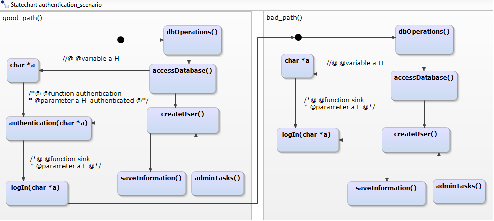
\includegraphics{styles/authentication_scenario.png}
	\caption{Authentication Scenario}
\end{figure}

\section{Declassification Scenario:}

\section{Sanitization Scenario:}
		\chapter{Related Work}

There are many annotation languages proposed until now for
extending the C type system [9], [13], [29], [30], [57] to be
used during run-time as a new language run-time for PHP and
Python [61] to annotate function interfaces [13], [29], [57], to
annotate models in order to detect information flow bugs [24]
to annotate source code files [46], [47], [56] or to annotate
control flows [13], [15], [29].The following annotation languages have made significant impact: Microsoft\'s SAL annotations [29] helped to detect more than 1000 potential security vulnerabilities in Windows
code [3]. In addition, several other annotation languages including FlowCaml [50], Jif [7], Fable [55], AURA [22] and FINE [54] express information flow related concerns.

UMLSec [23] is a model-driven approach that allows the
development of secure applications with UML. Compared with
our approach, UMLSec does neither automatic code
generation nor the annotations can be used for automated
constraints checking.

The detection of information flow errors [31] can be
addressed with dynamic analysis techniques [2], [16], [48],
static analysis techniques [17], [41], [51], [58], [60] (similar
to our approach with respect to static analysis of code and
tracking of data information flow) and hybrid techniques which
combine static and dynamic approaches [38]. Also, extended
static checking [10] (ESC) is a promising research area which
tries to cope with the shortage of not having certain program
run-time information.
The static code analysis techniques need to know which
parts of the code are: sinks, sources and which variables
should be tagged. A solution for tagging these elements in
source code is based on a pre-annotated library which contains
all the needed annotations attached to function declarations.
Leino [27] reports about the annotation burden as being very
time consuming and disliked by some programming teams.


 The studies rely on manually
written annotations while our annotation language is integrated
into two editors which are be used to annotate UML state
charts and C code by selecting annotations from a list and
without the need to memorize a new annotation language.

 Recently
taint modes integrated in programming languages as Camlbased FlowCaml [52], Ada-based SPARK Examiner [5] and the scripting. However, none of these annotation and programming languages have support for introducing information flow
restrictions in both models and the source code.
Splint [14], Flawfinder [59] and Cqual [49] are used to
detect information flow bugs in source code and come with
comprehensive user manuals describing how the annotation
language can be used in order to annotate source code.
iFlow [24] is used for detecting information flow bugs in
models and is based on modeling dynamic behavior of the
application using UML sequence diagrams and translating
them into code by analyzing it with JOANA [25]. In comparison with our approach these tools do not use the same
annotation language for annotating UML models and code.
Thus, a user has to learn to use two annotation languages
which can be perceived to be a high burden in some scenarios.


 Heldal et al. [18], [19] introduced an
UML profile that incorporates a decentralized label model [40]
into the UML. It allows the annotation of UML artifacts with
Jif [42] labels in order to generate Jif code from the UML
model automatically. However, the Jif-style annotation already
proved to be non-trivial on the code level [45], while [19]
notes that the actual automatic Jif code generation is still future
work. These approaches can not be used to annotate both UML
models and code. Moreover, these approaches lack of tools for
automated checking of previously imposed constraints.
		\chapter{Limitations}
The main limitations of this system are given below:
\begin{itemize}
	\item In UML state chart user can design function calls and statements of C/C++ language.
	
	\item Currently user have to model a real life system using region name good\_path() and bad\_path() or one of them in UML state chart editor. Otherwise code generator will not work.
	
	\item Now code generator generates only two files. One is .c file and another one is .h file.
	
	\item Code generator works with YAKINDU SCT editor.
	
	\item Static analysis engine works only in Ubuntu operating system.
	
	\item Code generator, UML statechart modeling developed in windows operating system.
	
	\item The simulation is not currently not working in selected scenarios in UML state chart editor.
	
	\item Now source, sink, authentication, declassification and santization types of function can be annotated. 
	
\end{itemize}
		
		\part[The 3rd Part]{Conclusion and Future Work}
		\chapter{Conclusion and Future Work}

In the conclusion and future work we will present the conclusion and possible future work of this research.

\section{Conclusion}
A keyword-based annotation language that can be used out of the box for annotating UML state charts and C code in two software development phases by providing two editors for inserting security annotations in order to detect information flow bugs automatically. It is evaluated on some sample programs and showed that this approach is applicable to real life scenarios.

Functions are used to declassify sensitive data because they are trusted to release information. Our work introduces a security-typed language. We annotate functions with security levels. Functions may be annotated with a high security level; this indicates they are trusted and permits them to serve as a safe mechanism for declassification.

Web applications perform a lot of critical tasks and
handle sensitive information. Even though there have been
a number of research efforts to identify the use of unvalidated input in web applications, little has been done
to characterize how sanitization is actually performed and
how effective it is in blocking web-based attacks. In case of desktop applications it is not easy to handle sensitive information. To handle these sensitive information and invalidate insecure input data a good approach to the evaluation of the sanitization process has been developed. Future work will focus on the analysis of type-based validation procedures.

Mechanisms such as access control, encryption, firewalls, digital
signatures and antivirus scanning do not address the fundamental
problem: tracking the flow of information in computing
systems. Run-time monitoring of operating-systems calls is
similarly of limited use because information-flow policies are
not properties of a single execution; in general, they require
monitoring all possible execution paths. On the other hand,
there is clear evidence of benefits provided by language-based
security mechanisms that build on technology for static analysis
and language semantics. Type systems are attractive for
implementing static security analyses. It is natural to augment
type annotations with security labels. Type systems allow for
compositional reasoning, which is a necessity for scalability
when applied to larger programs. Semantics-based models
are suitable for describing end-to-end policies such as
noninterference and its extensions. These models allow for a
precise formulation of the attacker's view of the system. This
view is described as a relation on program behaviors where
two behaviors are related if they are not distinguishable by
the attacker. Attackers of varying capabilities can be modeled
straightforwardly as different attacker views, and correspond
to different security properties. A number of further advantages are
associated with both security-type systems and semantics based
security. Compositionality is especially valuable in the
context of security properties.Compositionality
greatly facilitates correctness proofs for program analyses. If the recent
progress in language-based techniques for soundly enforcing
end-to-end confidentiality policies continues, the approach
may soon become an important part of standard security
practice.

Last but not least, it is a system which is usable for specifying information flow security constraints which can be used in the design and coding phase in order to detect information flow bugs.

\section{ Future Work}
In future it can be extended for source code editor as
a pop-up window based proposal editor used to add/retrieve
annotation to/from a library. The definition of new language
annotation tags should be possible from the same window by
providing two running modes (language extension mode and
annotation mode). The envisaged result is to reduce the gap
between annotations insertion/retrieval and the definition of
new language tags. This would help to create personalized
annotated libraries which can be collaboratively annotated if
needed.

Currently code generator, UML statechart modeling developed only for windows operating system. In future code generator, state chart editor should be implemented for other operating systems. Another avenue of future work lies in expanding the policy
language. It is currently very simple, but could be more expressive. For example, constraints could be added to indicate negative information flows. Policy analyses could also be used to determine whether separation of duties is maintained between two principals. When integrity is added to policy language, it could be expanded with robustness constraints. It is a general problem in language based security that there is too little experience with security-typed programming to help guide such research as designing the best form of declassification. We hope that our implementation of this mechanism will help to promote more practical experience with declassifiers which will be implemented in future research.



		
		% ---------------------------------------------------------------------------
		%
		% Appendix
		%
		% ---------------------------------------------------------------------------
		
		\part*{Appendix}
		\addcontentsline{toc}{part}{Appendix}
		
		\appendix %---------------------------------------
		
		\chapter{Appendix}
\section{Appendix A: Source Code Editor with Annotation Language}
\lstinputlisting[numbers=left,firstnumber=1,firstline=1]{sourceCode/MyDsl.xtext}

\section{Appendix B: C Code Generator}	
	\label{C_Code_Generator_Xtend_Code_Snippet}
	\lstinputlisting[numbers=left,firstnumber=1,firstline=1]{sourceCode/Types.xtend}
	
\section{Appendix C: Three Checkers in Static Analysis Engine}

\section{Appendix D: Sequence Diagram Generator}

		
	


  \clearemptydoublepage
  
	\bibliography{bibliography/literature}
	
 
\end{document}

